\documentclass[a4paper,12pt]{article}

\usepackage{mystyle}
\usepackage{gensymb}


\usepackage{scalerel}
\usepackage{stackengine}

\graphicspath{ {images/} }


\definecolor{violet}{RGB}{148, 0, 211}
\definecolor{red}{RGB}{183, 65, 14}
\definecolor{cyan}{RGB}{0, 153, 153}


% https://tex.stackexchange.com/a/101138/135045

\newcommand\widesim[1]{\ThisStyle{%
  \setbox0=\hbox{$\SavedStyle#1$}%
  \stackengine{-.1\LMpt}{$\SavedStyle#1$}{%
    \stretchto{\scaleto{\SavedStyle\mkern.2mu\sim}{.5150\wd0}}{.6\ht0}%
  }{O}{c}{F}{T}{S}%
}}

\newcommand{\BigMiddleThree}{\;\left|\vphantom{\begin{pmatrix} 0\\0\\0 \end{pmatrix}}\right.\;}


\author{Алексеев Василий}


\title{Семинар 1}
\date{3 + 7 февраля 2022}


\begin{document}
  \maketitle
  
  \tableofcontents

  \thispagestyle{empty}
  
  \newpage
  
  \pagenumbering{arabic}

  \section{``Refresher''}
    \noindent
    
    \textbf{Матрица} $A \in \RR^{m \times n} \equiv M$:
    \[
      A = \begin{pmatrix}
        a_{11} & \ldots & a_{1n}\\
        \vdots & \ddots & \vdots\\
        a_{m1} & \ldots & a_{mn}
      \end{pmatrix}, \quad a_{ij} \in \RR,\ i = 1 \ldots m,\ j = 1 \ldots n
    \]
    
    \textbf{Операции}:
    \begin{itemize}
      \item сложения матриц ($"{+}"\colon M \hm\times M \hm\to M$):
      \[
        C = A + B \Leftrightarrow c_{ij} = a_{ij} + b_{ij}
      \]
      
      \item умножения матрицы на число ($"{\cdot}"\colon \RR \hm\times M \hm\to M$):
      \[
        C = \alpha \cdot A \Leftrightarrow c_{ij} = \alpha \cdot a_{ij}
      \]
    \end{itemize}
    
    \textbf{Свойства} операций ($A, B, C \hm\in M$, $\alpha, \beta \hm\in R$):
    \begin{enumerate}
      \item $A + B = B + A$
      
      (коммутативность сложения)
      
      \item $(A + B) + C = A + (B + C)$
      
      (ассоциативность сложения)
      
      \item $\exists 0_{m\times n} \in M: A + 0_{m\times n} = 0_{m\times n} + A = A$
      
      (существование ``нейтральной'' матрицы относительно сложения)
      
      \item $\forall A\ \exists (-A): A + (-A) = (-A) + A = 0_{m\times n}$
      
      (существование ``обратной'' матрицы относительно сложения\footnote{Противоположная матрица.})
      
      \item $(\alpha \beta) A = \alpha (\beta A)$
      \item $1 \cdot A = A$
      \item $\alpha (A + B) = \alpha A + \alpha B$
      
      (дистрибутивность умножения относительно сложения матриц)
      
      \item $(\alpha + \beta) A = \alpha A + \beta A$
      
      (дистрибутивность умножения относительно сложения чисел)
    \end{enumerate}
    
    \textbf{Умножение} матриц:
    \[
      A_{m\times \bds p} B_{\bds p \times n} = C_{m\times n} \Leftrightarrow c_{ij} = \sum\limits_{k = 1}^p a_{ik} b_{kj},\ i = 1 \ldots m,\ j = 1 \ldots n
    \]
    
    \textbf{Свойства} (некоторые) операции умножения матриц (если не указано отдельно, то размеры матриц такие, чтоб операция была определена):
    \begin{enumerate}
      \item \sout{$A \cdot B = B \cdot A$}
      
      (в общем случае некоммутативна; даже может быть не определена, если матрицы переставить)
      
      \item $(A \cdot B) \cdot C = A \cdot (B \cdot C)$
      
      (ассоциативность умножения)
      
      \item $\exists E_{n\times n} \in \RR^{n\times n}: A_{n\times n} \cdot E_{n\times n} = E_{n\times n} \cdot A_{n\times n} = A_{n\times n}$
      
      (существование ``нейтральной'' матрицы относительно умножения в пространстве квадратных матриц $\RR^{n\times n}$)\footnote{Единичная матрица: $E = \diag(1, \ldots, 1).$}
      
      \item для любой квадратной \emph{невырожденной}\footnote{Матрица, строки которой линейно независимы.} матрицы $A \hm\in \RR^{n\times n}$ найдётся матрица $A^{-1} \hm\in \RR^{n\times n}$, такая что $A \hm\cdot A^{-1} = A^{-1} \hm\cdot A = E$
      
      (существование ``обратной'' матрицы относительно умножения)
    \end{enumerate}
    
    \textbf{Определитель} матрицы:
    \[
      \det\colon \RR^{n\times n} \to \RR
    \]
    
    Вычисление определителя:
    \[
      |a| = a
    \]
    \[
      \begin{vmatrix}
        a & b\\
        c & d
      \end{vmatrix} = ad - cb
    \]
    
    Разложение по первой строке при $A \hm\in \RR^{n\times n},\ n \hm\geq 2$ ($M_{1j}$~---~дополнительный минор элемента $a_{1j}$):
    \[
      \det(A) = \sum\limits_{j = 1}^n (-1)^{1 + j} a_{1j} M_{1j}
    \]
    
    
  \section{Ранг матрицы}
    Если квадратная матрица невырождена, то её строки линейно независимы.
    В общем же случае (вырожденная квадратная матрица или прямоугольная матрица) строки могут быть линейно зависимы.
    При этом, очевидно, можно (если матрица не нулевая) выбрать некоторое \emph{максимальное по количеству} подмножество строк матрицы так, чтобы выбранные строки оставались линейно независимы (\emph{строчный ранг}).
    Можно найти и максимальное по количеству подмножество линейно независимых столбцов матрицы (\emph{столбцовый ранг}).
    А можно найти максимальную по размеру невырожденную квадратную подматрицу (``просто'' \emph{ранг}).
    
    \begin{theorem}[О ранге матрицы]
      Ранг матрицы совпадает с её строчным и столбцовым рангами.
    \end{theorem}
    
    Поэтому можно ввести единое обозначение для ранга матрицы.
    Например:
    \[
      \Rg\colon \RR^{m\times n} \hm\to \RR
    \]
    
    Почему теорема ``работает''?
    Очевидно, строчный ранг матрицы равен столбцовому транспонированной.
    Поэтому можно сказать, что если доказать равенство строчного ранга и просто ранга, то со столбцовым будет ``аналогично''.
    Равенство же строчного ранга и ``просто'' ранга, возможно, поможет лучше понять картинка (\ref{fig:rangs}).
    
    \begin{figure}[h]
      \centering
    
      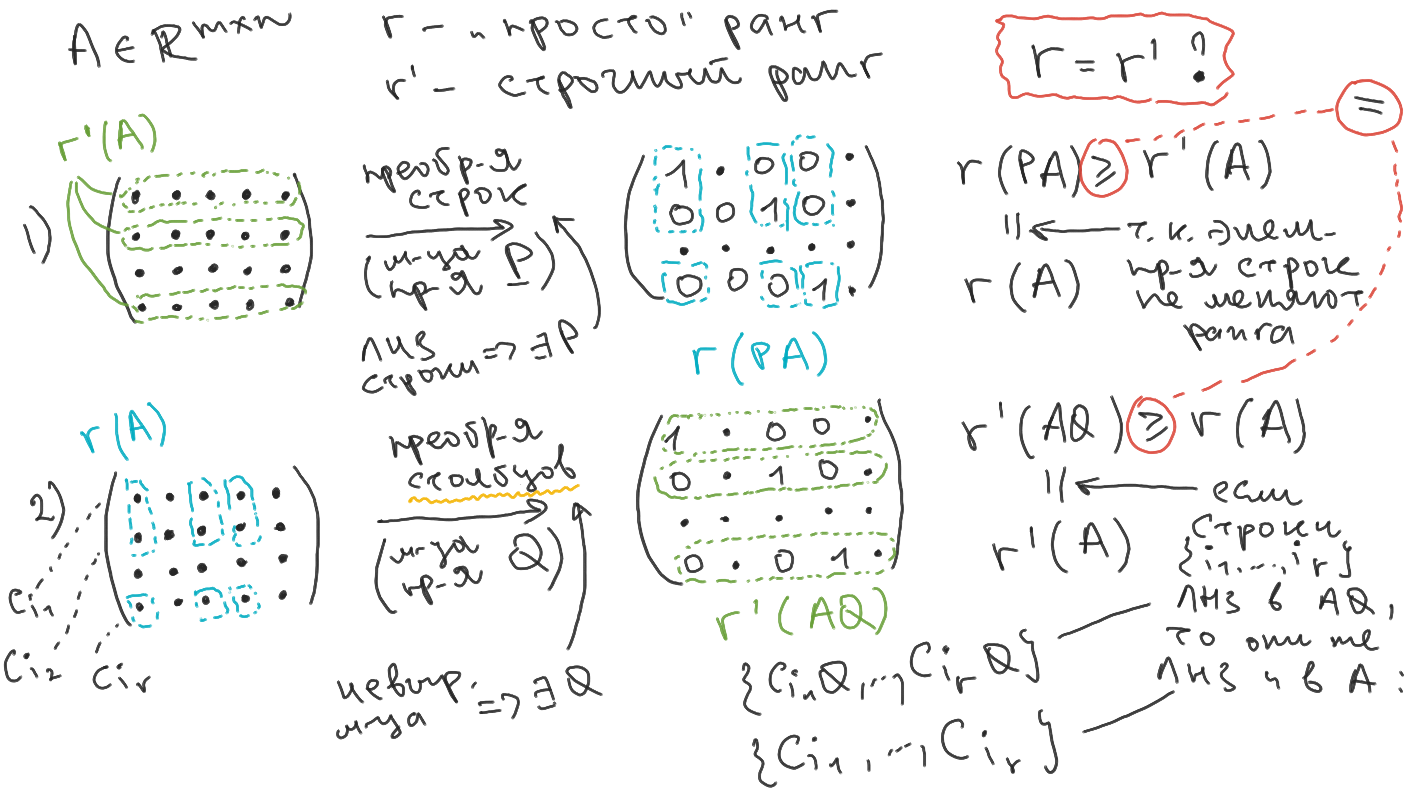
\includegraphics[width=0.8\columnwidth]{Rg.png}
    
      \caption{Картинка-пояснение к теореме о ранге матрицы: как можно "понять", почему равны строчный и просто ранги (почему в системе строк, которая максимальная по количеству система ЛНЗ строк, можно выбрать базисную подматрицу; и почему строки, в которых находится базисная подматрица, ЛНЗ~---~хотя про это, наверно, можно было и попроще догадаться...).}
      \label{fig:rangs}
    \end{figure}
  
    \begin{remark}
      Ранг матрицы не меняется при элементарных преобразованиях её строк (столбцов).
    \end{remark}
  
  
  
  \section{Задачи}
  
  
  \subsection{\# 15.45(2)}
  
  Вычислить обратную для матрицы
  \[
    A = \begin{pmatrix}
      2 & -1 & 0\\
      0 & 2 & -1\\
      -1 & -1 & 1
    \end{pmatrix}
  \]
  
  \begin{solution}
    Найдём обратную с помощью метода Гаусса.
    В основе метода лежат следующие понятия и ``наблюдения''.
    
    \begin{definition}
      Элементарные преобразования строк матрицы $A \in \RR^{m\times n}$:
      \begin{itemize}
        \item умножение строки на число, отличное от нуля;
        \item прибавление к строке другой строки;
        \item перестановка строк;
        \item прибавление к строке линейной комбинации других строк.
      \end{itemize}
    \end{definition}
    
    \begin{remark}
      Каждое элементарное преобразование строк матрицы $A \hm\in \RR^{m\times n}$ можно задать в виде невырожденной матрицы $S \hm\in \RR^{m \times m}$, которую надо умножить слева на $A$, чтобы провести преобразование.
      При этом матрица $S$ не зависит от $A$.
    \end{remark}
    
    \begin{remark}
      Если строки матрицы были линейно зависимы (независимы), то после элементарного преобразования строк они останутся линейно зависимы (независимы).
    \end{remark}
    
    \begin{remark}
      Для любой невырожденной матрицы $A$ существует последовательность элементарных преобразований строк $\{S_i\}_{i = 1}^N$, такая что она переводит матрицу $A$ в единичную:
      \[
        S_N \ldots S_1 A = E
      \]
    \end{remark}
    
    Вернёмся к решению задачи.
    Далее \textcolor{violet}{фиолетовым} цветом будем выделять элемент в столбце, с помощью которого будем занулять другие элементы в том же столбце.
    Те, которые зануляем на данном шаге, будем отмечать \textcolor{red}{красным} цветом.
    Когда столбец ``готов'' (остался один ненулевой~---~фиолетовый), переходим к другому столбцу и снова выбираем ненулевой элемент для ``зачищения столбца'', но \emph{из строчек, откуда ещё не выбирали}.
    Сначала можно занулять все элементы ниже главное диагонали (\emph{прямой ход} метода Гаусса), а потом~---~выше главной диагонали (\emph{обратный ход} метода Гаусса).
    
    \begin{equation*}
    \begin{split}
      &\left(
        \begin{matrix}
          2 & -1 & 0\\
          0 & 2 & -1\\
          -1 & -1 & 1
        \end{matrix}
        \BigMiddleThree
        \begin{matrix}
          1 & 0 & 0\\
          0 & 1 & 0\\
          0 & 0 & 1
        \end{matrix}
        \right)\\
      %
      \widesim{(1) \leftrightarrow (3)}\quad &\left(
        \begin{matrix}
          \textcolor{violet}{\bds{-1}} & -1 & 1\\
          \textcolor{red}{\bds 0} & 2 & -1\\
          \textcolor{red}{\bds 2} & -1 & 0
        \end{matrix}
        \BigMiddleThree
        \begin{matrix}
          0 & 0 & 1\\
          0 & 1 & 0\\
          1 & 0 & 0
        \end{matrix}
        \right)\\
      %
      \widesim{(3) = (3) + 2 \cdot (1)}\quad &\left(
        \begin{matrix}
          -1 & -1 & 1\\
          0 & 2 & -1\\
          0 & -3 & 2
        \end{matrix}
        \BigMiddleThree
        \begin{matrix}
          0 & 0 & 1\\
          0 & 1 & 0\\
          1 & 0 & 2
        \end{matrix}
        \right)\\
      %
      \widesim{(2) = (2) / 2}\quad &\left(
        \begin{matrix}
          -1 & -1 & 1\\
          0 & \textcolor{violet}{\bds 1} & -1/2\\
          0 & \textcolor{red}{\bds{-3}} & 2
        \end{matrix}
        \BigMiddleThree
        \begin{matrix}
          1 & 0 & 0\\
          0 & 1/2 & 0\\
          1 & 0 & 2
        \end{matrix}
        \right)\\
      %
      \widesim{(3) = (3) + 3 \cdot (2)}\quad &\left(
        \begin{matrix}
          -1 & -1 & \textcolor{red}{\bds{1}}\\
          0 & 1 & \textcolor{red}{\bds{-1/2}}\\
          0 & 0 & \textcolor{violet}{\bds{1/2}}
        \end{matrix}
        \BigMiddleThree
        \begin{matrix}
          0 & 0 & 1\\
          0 & 1/2 & 0\\
          1 & 3/2 & 2
        \end{matrix}
        \right)\\
      %
      \widesim{\substack{(1) = (1) - 2 \cdot (3)\\(2) = (2) + (3)}}\quad &\left(
        \begin{matrix}
          -1 & \textcolor{red}{\bds{-1}} & 0\\
          0 & \textcolor{violet}{\bds{1}} & 0\\
          0 & 0 & 1/2
        \end{matrix}
        \BigMiddleThree
        \begin{matrix}
          -2 & -3 & -3\\
          1 & 2 & 2\\
          1 & 3/2 & 2
        \end{matrix}
        \right)\\
      %
      \widesim{\substack{(1) = (1) + (2)\\(3) = 2 \cdot (3)}}\quad &\left(
        \begin{matrix}
          -1 & 0 & 0\\
          0 & 1 & 0\\
          0 & 0 & 1
        \end{matrix}
        \BigMiddleThree
        \begin{matrix}
          -1 & -1 & -1\\
          1 & 2 & 2\\
          2 & 3 & 4
        \end{matrix}
        \right)\\
      %
      \widesim{(1) = -1 \cdot (1)}\quad &\left(
        \begin{matrix}
          1 & 0 & 0\\
          0 & 1 & 0\\
          0 & 0 & 1
        \end{matrix}
        \BigMiddleThree
        \begin{matrix}
          1 & 1 & 1\\
          1 & 2 & 2\\
          2 & 3 & 4
        \end{matrix}
        \right)
    \end{split}
    \end{equation*}
    
    Таким образом,
    \[
      A^{-1} = \begin{pmatrix}
        1 & 1 & 1\\
        1 & 2 & 2\\
        2 & 3 & 4
      \end{pmatrix}
    \]
    
    Можно (стоит) проверить:
    \[
      AA^{-1} = \begin{pmatrix}
        2 & -1 & 0\\
        0 & 2 & -1\\
        -1 & -1 & 1
      \end{pmatrix}
      \cdot \begin{pmatrix}
        1 & 1 & 1\\
        1 & 2 & 2\\
        2 & 3 & 4
      \end{pmatrix}
      = \begin{pmatrix}
        1 & 0 & 0\\
        0 & 1 & 0\\
        0 & 0 & 1
      \end{pmatrix}
    \]
    
    Почему преобразования строк у ``сдвоенной'' матрицы позволило найти $A^{-1}$?
    Каждый шаг метода Гаусса можно рассматривать как умножение слева на некоторую невырожденную матрицу $S_i$, задающую соответствующее элементарное преобразование строк:
    \[
      \bigl(A \mid E\bigr) \to \bigl(S_1 A \mid S_1 E\bigr) \to \ldots
      \to \bigl(\overbrace{S_N \ldots S_1 A}^{E} \mid \overbrace{S_N \ldots S_1 E}^{B}\bigr)
    \]
    где единичная матрица $E \hm= S_N \ldots S_1 A$~---~то, что стремимся получить слева, справа же получается матрица $B \hm= S_N \ldots S_1 E \hm= S_n \ldots S_1$.
    Выходит, $E \hm= BA$, что равносильно\footnote{Можно показать, что при $BA \hm= E$ обязательно выполняется также и $AB \hm= E$} тому, что $B \hm= A^{-1}$.
    
    \bigskip
    
    \paragraph{Отступление.}
    
    Найдём интереса ради какую-нибудь $S_i$.
    Например, $S_1$, которая задаёт перестановку строк.
    Правда, перестановка строк~---~не совсем элементарное преобразование.
    Разложим его сначала на элементарные.
    
    Мы хотим задать преобразование перестановки строк (первой и третьей):
    \[
      \begin{pmatrix}
        2 & -1 & 0\\
        0 & 2 & -1\\
        -1 & -1 & 1
      \end{pmatrix}
      \longrightarrow \begin{pmatrix}
        -1 & -1 & 1\\
        0 & 2 & -1\\
        2 & -1 & 0
      \end{pmatrix}
    \]
    
    Это преобразование можно представить как композицию преобразований (над-под каждой стрелочкой обозначено элементарное преобразование и его матрица\footnote{Матрица, которую можно получить,например, из единичной, проведя над её строками аналогичное преобразование.}):
    \begin{equation*}
    \begin{split}
      &\begin{pmatrix}
        2 & -1 & 0\\
        0 & 2 & -1\\
        -1 & -1 & 1
      \end{pmatrix}\\
      \xrightarrow[(3) = (3) + (1)]{\left(\begin{smallmatrix}1 & 0 & 0\\0 & 1 & 0\\1 & 0 & 1\end{smallmatrix}\right)}\quad &\begin{pmatrix}
          2 & -1 & 0\\
          0 & 2 & -1\\
          1 & -2 & 1
        \end{pmatrix}\\
      \xrightarrow[(1) = (1) - (3)]{\left(\begin{smallmatrix}1 & 0 & -1\\0 & 1 & 0\\0 & 0 & 1\end{smallmatrix}\right)}\quad &\begin{pmatrix}
          1 & 1 & -1\\
          0 & 2 & -1\\
          1 & -2 & 1
        \end{pmatrix}\\
      \xrightarrow[(3) = (3) + (1)]{\left(\begin{smallmatrix}1 & 0 & 0\\0 & 1 & 0\\1 & 0 & 1\end{smallmatrix}\right)}\quad &\begin{pmatrix}
          1 & 1 & -1\\
          0 & 2 & -1\\
          2 & -1 & 0
        \end{pmatrix}\\
      \xrightarrow[(1) = -1 \cdot (1)]{\left(\begin{smallmatrix}-1 & 0 & 0\\0 & 1 & 0\\0 & 0 & 1\end{smallmatrix}\right)}\quad &\begin{pmatrix}
          -1 & -1 & 1\\
          0 & 2 & -1\\
          2 & -1 & 0
        \end{pmatrix}
    \end{split}
    \end{equation*}
    
    И в итоге, $S_1$, задающая первую перестановку строк:
    \[
      S_1 = \begin{pmatrix}
          -1 & 0 & 0\\
          0 & 1 & 0\\
          0 & 0 & 1
        \end{pmatrix}
      \cdot \begin{pmatrix}
          1 & 0 & 0\\
          0 & 1 & 0\\
          1 & 0 & 1
        \end{pmatrix}
      \cdot \begin{pmatrix}
          1 & 0 & -1\\
          0 & 1 & 0\\
          0 & 0 & 1
        \end{pmatrix}
      \cdot \begin{pmatrix}
          1 & 0 & 0\\
          0 & 1 & 0\\
          1 & 0 & 1
        \end{pmatrix}
      = \ldots
    \]
  \end{solution}
  
  
  
  \subsection{\# 15.65(3)}
  
  \[
    \begin{pmatrix}
      2 & 1\\
      1 & 1
    \end{pmatrix} X = \begin{pmatrix}
      10\\
      17
    \end{pmatrix}
  \]
  
  \begin{solution}
    Пусть $A \hm\equiv \left(\begin{smallmatrix}
      2 & 1\\
      1 & 1
    \end{smallmatrix}\right)$ и $b \hm\equiv \left(\begin{smallmatrix}
      10\\
      17
    \end{smallmatrix}\right)$.
    
    Какая размерность у матрицы $X$?
    Обозначим размерность матрицы $X$ за $m \hm\times n$ (число строк и число столбцов).
    Тогда имеем:
    \[
      A_{\textcolor{red}{2} \times {\bds 2}} X_{{\bds m} \times \textcolor{cyan}{n}} = b_{\textcolor{red}{2} \times \textcolor{cyan}{1}}
    \]
    
    Поэтому $m \hm= 2$ и $n \hm= 1$.
    
    Также можно заметить, что матрица $A$, которая левый множитель, невырождена.
    
    Как искать $X$?
    
    \bigskip
    
    \paragraph{Способ I: ``По-простому''.}
    
    Пусть $X \hm= \left(\begin{smallmatrix}x \\ y\end{smallmatrix}\right)$.
    Тогда матричное уравнение $AX \hm= b$ равносильно системе из двух скалярных уравнений:
    \[
      \left\{
        \begin{aligned}
          &2x + y = 10\\
          &x + y = 17
        \end{aligned}
      \right.
    \]
    
    Которую можно решить, например, методом Крамера (матрица системы невырождена):
    \[
      \left\{
        \begin{aligned}
          &x = \frac{\left|\begin{smallmatrix}10 & 1 \\ 17 & 1\end{smallmatrix}\right|}{\left|\begin{smallmatrix}2 & 1 \\ 1 & 1\end{smallmatrix}\right|} = \frac{10 - 17}{\det(A)}\\
          &y = \frac{\left|\begin{smallmatrix}2 & 10 \\ 1 & 17\end{smallmatrix}\right|}{\left|\begin{smallmatrix}2 & 1 \\ 1 & 1\end{smallmatrix}\right|} = \frac{2 \cdot 17 - 10}{\det(A)}
        \end{aligned}
      \right.
    \]
    
    
    \medskip
    
    \paragraph{Способ II: ``В контексте темы''.}

    Чтобы найти $X$, можно умножить \emph{слева} обе части уравнения на обратную к матрице-множителю:
    \[
    \underbrace{\begin{pmatrix}
      2 & 1\\
      1 & 1
    \end{pmatrix}^{-1}
    \begin{pmatrix}
      2 & 1\\
      1 & 1
    \end{pmatrix}}_{E} X = \begin{pmatrix}
      2 & 1\\
      1 & 1
    \end{pmatrix}^{-1}
    \begin{pmatrix}
      10\\
      17
    \end{pmatrix}
  \]
  
  В итоге, после нахождения обратной, например, по формуле, получаем:
  \[
    X = \frac{1}{\det(A)} \cdot \begin{pmatrix}
      1 & -1\\
      -1 & 2
    \end{pmatrix}
    \begin{pmatrix}
      10\\
      17
    \end{pmatrix}
    = \frac{1}{\det(A)} \cdot \begin{pmatrix}
      10 - 17\\
      2 \cdot 17 - 10
    \end{pmatrix}
  \]
  \end{solution}
  
  
  \bigskip
  
  \paragraph{Заметка на полях $1$.}
  
  Можно было не умножать обе части уравнения на $A^{-1}$, а представить правую часть как $b \hm= AA^{-1}b$ и перенести влево, вынеся потом $A$ за скобку. (Почему можно потом приравнять нулю то, что останется в скобках: $X \hm- A^{-1}b$?)
  
  \medskip
  
  \paragraph{Заметка на полях $2$.}
  
  Матрица $A$ была невырожденной.
  Посмотрим, что могло бы быть, если бы $A$ была вырожденной.
  Например, так:
  \[
    \begin{pmatrix}
      1 & 1\\
      1 & 1
    \end{pmatrix} X = \begin{pmatrix}
      10\\
      17
    \end{pmatrix}
  \]
  
  Очевидно, в таком случае решений нет.
  
  Или так (поменяем ещё столбец справа):
  \[
    \begin{pmatrix}
      1 & 1\\
      1 & 1
    \end{pmatrix} X = \begin{pmatrix}
      10\\
      10
    \end{pmatrix}
  \]
  
  Сводя к системе скалярных уравнений, получаем следующее решение:
  \[
    X = \begin{pmatrix}
      t\\
      10 - t
    \end{pmatrix}
    = \begin{pmatrix}
      0\\
      10
    \end{pmatrix} + \begin{pmatrix}
      1\\
      -1
    \end{pmatrix} t, \quad t \in \RR
  \]
  
  То есть очевидно, что в данном случае решение не просто есть, а их бесконечно много\footnote{Умножение матрицы $A$ справа на столбец $X$ равносильно составлению столбца, являющегося линейной комбинацией столбцов $A$ с коэффициентами, записанными в столбец $X$. Очевидно, в рассматриваемом случае столбец $b$ можно разложить по столбцам $A$, хоть они и линейно зависимы.}.
  
  
  
  \subsection{\# 16.19(3)}
  
  \[
    A = \begin{pmatrix}
      1 & 1 & 1\\
      1 & \alpha & \alpha\\
      1 & \alpha^2 & \alpha^2
    \end{pmatrix}
  \]
  \[
    \Rg A = \?
  \]
  
  \begin{solution}
  
    Рассмотрим пару способов решения.
    
    \paragraph{Способ I: ``Наблюдения''.}
    
    В матрице $A$ есть ненулевые элементы, поэтому $\Rg A \hm\geq 1$.
    Второй и третий столбцы матрицы $A$ линейно зависимы, то есть матрица $A$ вырождена, поэтому $\Rg A \hm< 3$.
    Имеет смысл далее рассмотреть систему из первого и, например, второго столбцов матрицы $A$.
    Они линейно зависимы при $\alpha \hm= 1$ (то есть $\Rg A \hm= 1$).
    При всех других $\alpha$ они линейно независимы  (то есть $\Rg A \hm= 2$).
  
    \medskip
    
    \paragraph{Способ II: ``Ещё раз метод Гаусса''.}
    
    Чтобы найти ранг матрицы, можно методом Гаусса привести её к упрощённому виду (то есть ``пытаться'' преобразованиями строк привести матрицу $A \hm\in \RR^{m\times n}$ к единичной: если матрица квадратная и вырожденная или прямоугольная, то некоторые строки в общем случае могут оказаться нулевыми, то есть на очередном шаге метода Гаусса может не получиться найти ненулевой элемент, с помощью которого надо было бы занулять ``лишние'').
    Первым преобразованием можно вычесть первую строку из второй и третьей:
    \[
      \begin{pmatrix}
        1 & 1 & 1\\
        1 & \alpha & \alpha\\
        1 & \alpha^2 & \alpha^2
      \end{pmatrix}
      \longrightarrow
      \begin{pmatrix}
      1 & 1 & 1\\
      0 & \alpha - 1 & \alpha - 1\\
      0 & \alpha^2 - 1 & \alpha^2 - 1
    \end{pmatrix}
    \]
    
    Далее метод Гаусса продолжать сразу нельзя, потому что не понятно, нулевые вторая и третья строки или нет.
    Например, следующим шагом метода Гаусса могла бы быть ``чистка второго столбца'', но для этого во второй или третьей строчке должен быть ненулевой элемент во втором столбце.
    \[
      \alpha = 1 \Rightarrow A = \begin{pmatrix}
        1 & 1 & 1\\
        0 & 0 & 0\\
        0 & 0 & 0
      \end{pmatrix} \Rightarrow \Rg A = 1
    \]
    
    Пусть $\alpha \hm{\not=} 1$.
    Тогда вторая строчка ненулевая, и можно её (и третью строчку тоже) поделить на $\alpha - 1$:
    \[
      \begin{pmatrix}
        1 & 1 & 1\\
        0 & \alpha - 1 & \alpha - 1\\
        0 & \alpha^2 - 1 & \alpha^2 - 1
      \end{pmatrix}
      \longrightarrow
      \begin{pmatrix}
        1 & 1 & 1\\
        0 & 1 & 1\\
        0 & \alpha + 1 & \alpha + 1
      \end{pmatrix}
    \]
    
    Вне зависимости от того, нулевая третья строчка или нет, её можно занулить, вычтя с нужным коэффициентом вторую.
    То есть
    \[
      \begin{pmatrix}
        1 & 1 & 1\\
        0 & 1 & 1\\
        0 & \alpha + 1 & \alpha + 1
      \end{pmatrix}
      \longrightarrow
      \begin{pmatrix}
        1 & 1 & 1\\
        0 & 1 & 1\\
        0 & 0 & 0
      \end{pmatrix}
      \longrightarrow
      \begin{pmatrix}
        1 & 0 & 0\\
        0 & 1 & 1\\
        0 & 0 & 0
      \end{pmatrix}
    \]
    
    Привели матрицу $A$ к упрощённому виду (в первых строках можно найти подматрицу единичной матрицы, а остальные строки~---~нулевые).
    Ранг у упрощённой матрицы равен двум.
    Поэтому и $\Rg A \hm= 2$ (при $\alpha \hm{\not=} 1$).
  \end{solution}
\end{document}
